\documentclass[11pt,fleqn]{article}

\setlength {\topmargin} {-.15in}
\setlength {\textheight} {8.6in}

\usepackage{amsmath}
\usepackage{amssymb}
\usepackage{color}
\usepackage{tikz}
\usetikzlibrary{automata,positioning,arrows}
\usepackage{diagbox}
\usepackage{stackrel}

\newcommand{\be}{\begin{enumerate}}
\newcommand{\ee}{\end{enumerate}}

\begin{document}


\textbf{Exercise 3.2.15}
\begin{center}
	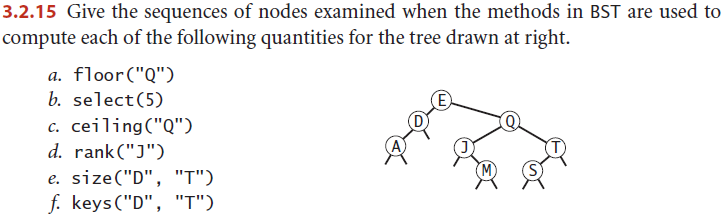
\includegraphics[scale=1]{3.2.15.png}
\end{center}

\textbf{Solution:}
\be
	\item floor("Q"). Recall floor represents largest local key $\le$ given key. SOLN: E,Q
	
	\item select(5): Recall selection is the process of seeking the key node of the rank. The key k such that precisely k other keys in BST are smaller. So it checks right sub-tree of E as has more than 5 keys. Two on the left subtree, 2 on the right, and itself counts as 1). Therefore, the sequence checked for select(5) is E,Q
	
	\item Ceiling("Q"). Recall Ceiling is the smallest local key $\ge$ given key. Ceiling checks E,Q $AND$ stops as smallest key $\ge$ given key(Q) since Q itself is smallest possible value we can get.
	
	\item rank("J"): Rank is somewhat similar to floor, except returns the number of nodes that satisfy a given condition. So finds the number of child nodes that are less than a given node. Goes through E,Q then J and then finds number of child nodes of J.  Therefore, the sequence checked is: E,Q,J
	
	\item size("D", "T"): E,D,Q,J,M,S
	\item keys("D", "T"): E,D,Q,J,M,S
\ee



\end{document}
